\chapter{Posicionamento do trem de pouso}

\begin{figure}
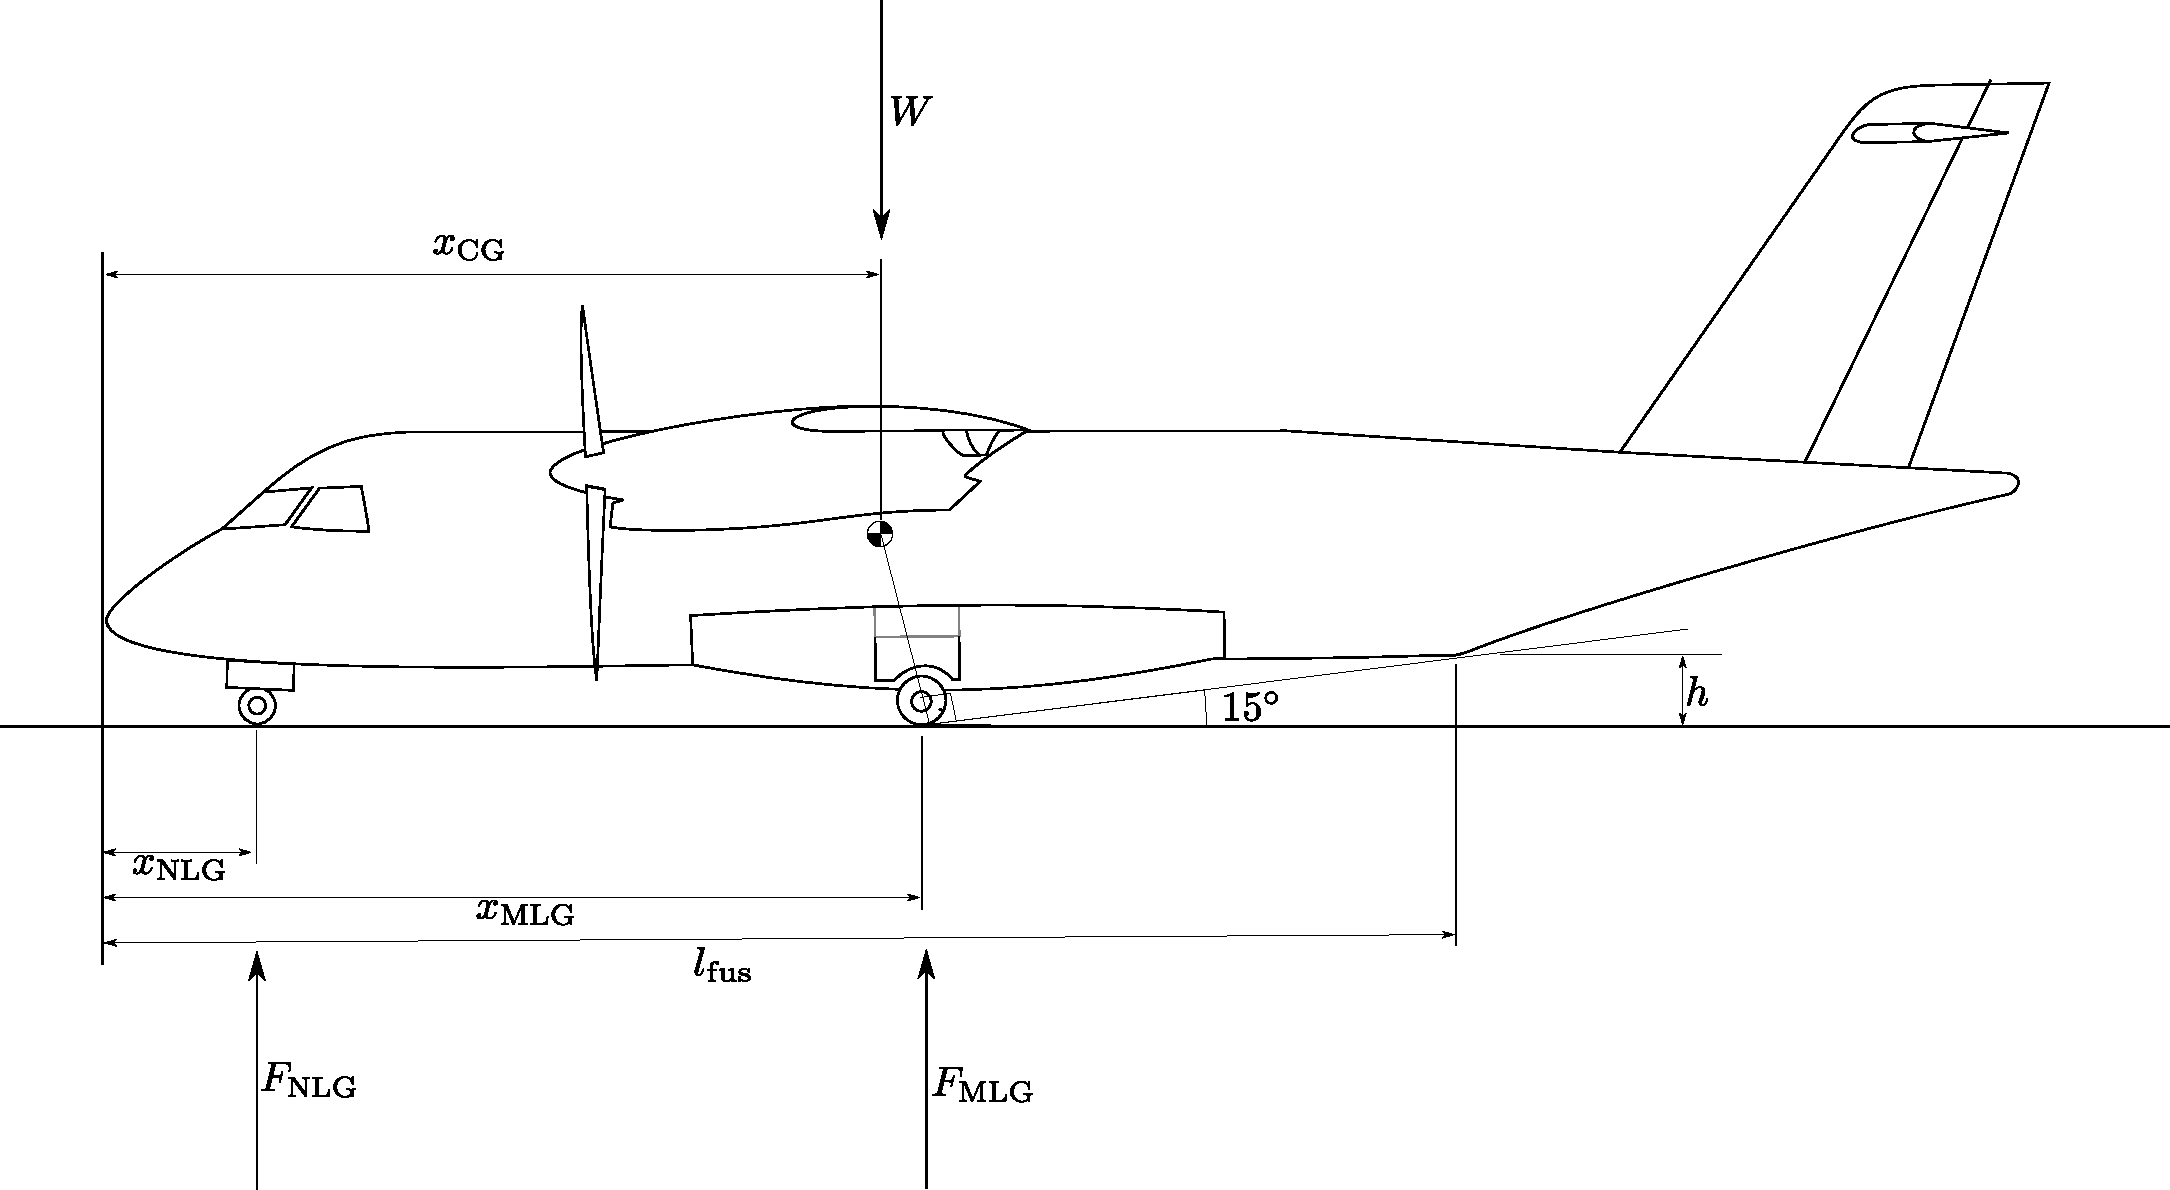
\includegraphics[width=\textwidth]{tdp.pdf}
\caption{Geometria do trem de pouso}
\label{fig:tdp}
\end{figure}

A geometria básica do trem de pouso triciclo está esboçada na \autoref{fig:tdp}. De acordo com~\cite{gudmundsson}, é desejável que a aeronave consiga desenvolver um ângulo de ataque de pelo menos \ang{15} durante a decolagem. Para isso, é necessário que a altura do trem de pouso permita seja pelo menos 
\begin{equation} 
h=(l_\text{fus}-x_\text{MLG})\tan\ang{15}
\end{equation}
onde $l_\text{fus}=20\si{m}$ é o comprimento da parte pressurizada da fuselagem e $x_\text{MLG}$ é a posição horizontal do trem de pouso principal. Apenas a parte pressurizada da fuselagem é importante para esse cálculo porque apenas ela é cilíndrica. A parte não pressurizada pode ser feita em forma de cone de modo que não atinja o solo na rotação.

Além disso, quanto o avião está rotacionado de \ang{15} com o CG traseiro, o peso deve estar na linha do trem de pouso principal, o que leva a equação
\begin{equation}
x_{\text{MLG}} = {x{_\text{CG}}}_{\max} + (d_{\text{fus}}/2 +h) \tan\ang{15}
\end{equation}
onde $d_\text{fus}=2,1\si{m}$ é o diâmetro da fuselagem.

Resolvendo esse sistema, temos a posição do trem de pouso principal
\begin{align}
x_\text{MLG} &= 14,664\si{m}\\
h            &= 1,430 \si{m} 
\end{align}

De acordo com os requisitos da FAR~25, a distância mínima entre a hélice e o solo deve ser de 7\si{in}. Como o diâmetro da fuselagem é de 2,1m e o raio da hélice é de 2,108\si{m}, a altura mínima do trem de pouso é de 178,6\si{mm}. A altura calculada acima cumpre esse requisito com folga.

Para a posição do trem de pouso do nariz, \cite{gudmundsson} recomenda que a carga no nariz seja de 10 a 20\% do peso da aeronave. Por equilibrio de forças e momentos na \autoref{fig:tdp}
\begin{align}
W             &= F_\text{NLG} + F_\text{MLG} \\
x_\text{CG} W &= x_\text{NLG} F_\text{NLG} + x_\text{MLG} F_\text{MLG}
\end{align}

Definindo a carga adimensional no trem de pouso de nariz pelo parâmetro $\lambda \triangleq \frac{F_\text{NLG}}{W}$, temos que a posição do trem de pouso de nariz é obtida por
\begin{equation}
x_\text{NLG} = \frac{x_\text{CG} - x_\text{MLG}(1-\lambda)}{\lambda}
\end{equation}
e inversamente a carga normalizada no nariz pode ser obtida por
\begin{equation}
\lambda = \frac{x_\text{MLG} - x_\text{CG}}{x_\text{MLG}-x_\text{NLG}}
\end{equation}

Projetando a posição do trem de pouso para que ela fique responsável por 15\% do peso na posição média do CG de 12,5m, obtêm-se
\begin{equation}
x_\text{NLG} = 0,235\si{m}
\end{equation}

Isso faz com que a carga máxima no trem de pouso de nariz seja de 25\% do peso com o CG mais dianteiro e a mínima seja 4,6\% do peso com o CG mais traseiro. Apesar desses intervalo ser maior que o recomendado por \cite{gudmundsson}, a forma de reduzí-lo é limitando o passeio do CG, o que não é desejável.

Por conveniência, o posicionamento básico do trem de pouso definido neste capítulo está resumido abaixo

\begin{align*}
x_\text{MLG} &= 14,664\si{m}\\
x_\text{NLG} &= 0,235\si{m}\\
h            &= 1,430 \si{m} 
\end{align*}


